
\emph{Deep Learning} (DL), também conhecido como Aprendizado Profundo, é uma subárea específica de ML que enfatiza o aprendizado através de sucessivas camadas de representações cada vez mais significativas dos dados submetidos. Estas representações são quase sempre obtidas atráves de redes neurais profundas \cite{chollet}. De acordo com Heaton, qualquer RNA com mais de duas camadas ocultas é, em sua essência, considerada profunda \cite{heaton}. O DL tem obtido um êxito incrível em endereçar problemas de visão computacional e processamento de linguagem natural. Estes algoritmos não só ultrapassaram outras variedades de algoritmos de ML, como também pleiteam a eficácia na classificação alcançada por seres humanos \cite{buduma}.

Os motivos para o corrente sucesso do DL podem ser exemplificados pela grande quantidade de dados disponíveis -- como a base de dados \emph{ImageNet}, organizada conforme a hierarquia \emph{WordNet} e que disponibiliza imagens para pesquisadores ao redor do mundo \cite{imagenet} -- e o custo relativamente baixo de Unidades de Processamento Gráfico (GPUs), que são utilizadas para uma computação numérica muito mais eficiente. Grandes companhias do ramo tecnológico utilizam técnicas de DL diariamente para a análise de enormes quantidades de dados. Entretanto, esta especiliadade não é mais limitada somente ao domínio acadêmico e industrial, ela tornou-se parte integrante da produção de softwares modernos disponibilizados aos consumidores \cite{gulli}.

O DL reúne um conjunto de técnicas e modelos que podem ser aplicados a tarefas de aprendizado supervisionado e não-supervisionado, nas quais as redes neurais convolucionais se destacam expressivamente. A próxima seção descreve os pontos principais relacionados a este tipo de RNA.

\subsubsection{Redes Neurais Convolucionais}
\label{subsubsec:cnns}

As \emph{Redes Neurais Convolucionais} (CNNs, do inglês \emph{Convolutional Neural Networks}) são uma categoria de redes neurais profundas, \emph{feedforward}, que comprovaram ser extremamente bem-sucedidas no ramo de visão computacional \cite{khan}. O termo denominado a estas redes, vem do seu aproveitamento da operação matemática chamada convolução, um tipo especializado de operação linear \cite{goodfellow}.



\begin{figure}[h!]
\centering
\caption{A relação entre a visão humana, visão computacional, ML, DL e CNNs. Adaptado de: \cite{khan}.}
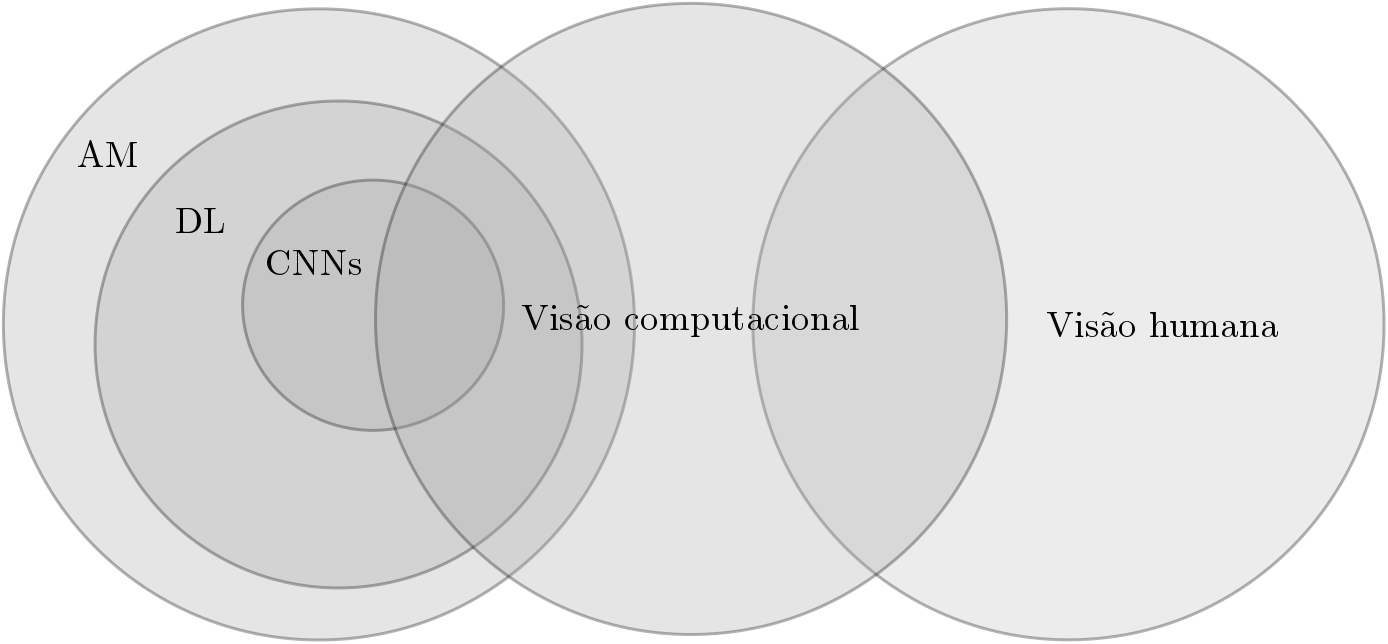
\includegraphics[height=4cm]{imgs/areas-ia}
\label{fig:areas-ia}
\end{figure}

% Convolução
% Pooling
% Dropout (Pegar imagens sobre Dropout na pagina favoritada)
% Arquiteturas canônicas


\subsubsection{Arquiteturas canônicas de Redes Neurais Convolucionais}
\label{subsubsec:arq-cnns}
